\documentclass{article}
\usepackage{color}
\usepackage{placeins}
\usepackage{listings}
\usepackage{graphicx}
\usepackage{xcolor}
\usepackage{amsmath}
\usepackage{subcaption}
\usepackage{cleveref}
\usepackage{array}
\usepackage{geometry}[margins=1in]
\setlength{\parskip}{4pt plus 2pt}
\setlength{\parindent}{0pt}
%\pagecolor[rgb]{0,0,0} %black
%\color[rgb]{1,1,1} %grey
\lstset{language=C++,
keywordstyle=\color{blue},
stringstyle=\color{red},
commentstyle=\color{green},
morecomment=[l][\color{magenta}]{\#},
breaklines=true,
breakatwhitespace=true,
numbers=left
}
\title{Assignment \#6}
\author{Asbjørn Bonefeld Preuss,\\ Daniel Lomholt Christensen,\\ Elie Cueto}
\date{March 2024}

\renewcommand{\thesection}{Task \#\arabic{section}}
\renewcommand{\thesubsection}{\arabic{section}.\arabic{subsection}}
\begin{document}
\maketitle
\section{MPI parallelise the program}
The initial calls to start up MPI were already included in the code, letting us focus solely on the parallelization. 

Firstly, we want to split up the world into sections, such that each MPI rank can work on its own section. The best way to do this splitting up is the way which minimizes the amount of data that has to be communicated between each rank, equivalent to minimizing the circumference of each domain. We therefore find the 2D decomposition that results in each section being as square-like as possible, on lines 250-289.

With the number of ranks in each dimension we can now set up an MPI cartesian system for our processors, which will be very convenient when exchanging information between neighbouring ranks. This is done on lines 293-304. 

Then, on lines 306-318, we determine the size and location of the section of the world each rank is assigned. This is complicated a bit by the fact that each section is not always the exact same size, depending on whether the number of cells in each direction is divisible by the number of ranks in each direction, but we do find a solution.

The next thing to do is to define the datatypes to use when exchanging ghost cells. We use MPI\_Type\_create\_subarray for both the horizontal and vertical exchanges, so that when doing the exchange, each rank only has to send one element of either horiz\_type or vert\_type to each of its its neighbours. These are defined on lines 340-365. Now we can begin the simulation.

Most of the simulation proceeds as normal, only the ghost cell exchanges were changed. Here we make use of the MPI\_Neighbor\_alltoallw function, which allowed us to send all the ghost cells between ranks, neatly packaged in the subarray types, in two lines. Then, after each completed timestep, we add an MPI\_Barrier.  This is moslty just a precaution, as it shouldn't be necessary to include, but as each rank will wait for all the others to arrive in the ghost cell exchange, it should also not cause any significant decrease in performance. With this the main part of the code runs in parallel. 

Next step is to gather all the data properly rank 0, so it can be written out to a file. Here, out solution is not the most elegant. Before the simulation starts, we use MPI\_Gather to collect the sizes of all the ranks' sections on rank 0, so that later, when rank 0 has to gather the whole world, we can use MPI\_Gatherv to collect all the world data. The inelegant part lies in the fact that we take all the world cells on each rank, convert them to a 1D vector, and collect them all as a 1D vector on rank 0, one flattened world after another. This is then written out in a way that, when loaded in with the visual.ipynb notebook, it does not look sensible. Here, however, we reformat the data, and the expected temperature map of the world is recovered. 

Finally, we want to parallelize the checksum calculation as well as the min, max, and mean calculations. We do this by first letting each rank calculate its own sum - or minimum or maximum - and then doing a reduction onto rank 0, which is then left with the global sum, minimum or maximum. In the mean case, rank 0 then divides the total sum by the global world size to find the global mean. Doing this, we reproduce the values on the sequential version.


%The calls to start up MPI have already been added to the parallel version of the program. Your task is
%to complete the parallelisation. This entails deciding on a domain decomposition, exchanging data
%between processes where appropriate, making sure that diagnostics used to check correctness are
%computed correctly, and collecting data on rank=0 when writing our I/O. Besides your implementation
%submitted as the code and in pdf, you also submit a report through Absalon. In the report, you should
%explain how you have parallelised the program. Remember to check and show that you get the same
%checksum and stats running on different number of cores. The 7 points are distributed as follows:
%• Working parallel checksum and stats routines (up to 1 point)
%• One dimensional slab domain decomposition of the integration loop (up to 2 points)
%• Functioning I/O (up to 2 points)
%• Two-dimensional domain decomposition of the problem (up to 2 points)
%There can be extra points for elegant solutions or going beyond the minimum (e.g. looking at hybrid
%OpenMP + MPI)
\section{Strong scaling using SLURM}
The parallelized program was run on N cores, where N goes from 1 to 192. This was done for both the medium and small, but the large was only run on 1 to 200 cores, as this took longer to run. The effectivity for each run was calculated, and Amdahls law was fitted to the data points for the small, medium, and large results.
These fits and results can be seen on figure \ref{fig:Efficiency_plot}. 

It is clear, that the exchange of ghost lines take too large an overhead for the small model, making the program less efficient when split up between more than 30 cores. In contrast the scaling of the medium model shows that the efficiency increases, until a new node has to be used. After this, the overhead costs also make the program run slower.


\begin{figure}
    \centering
    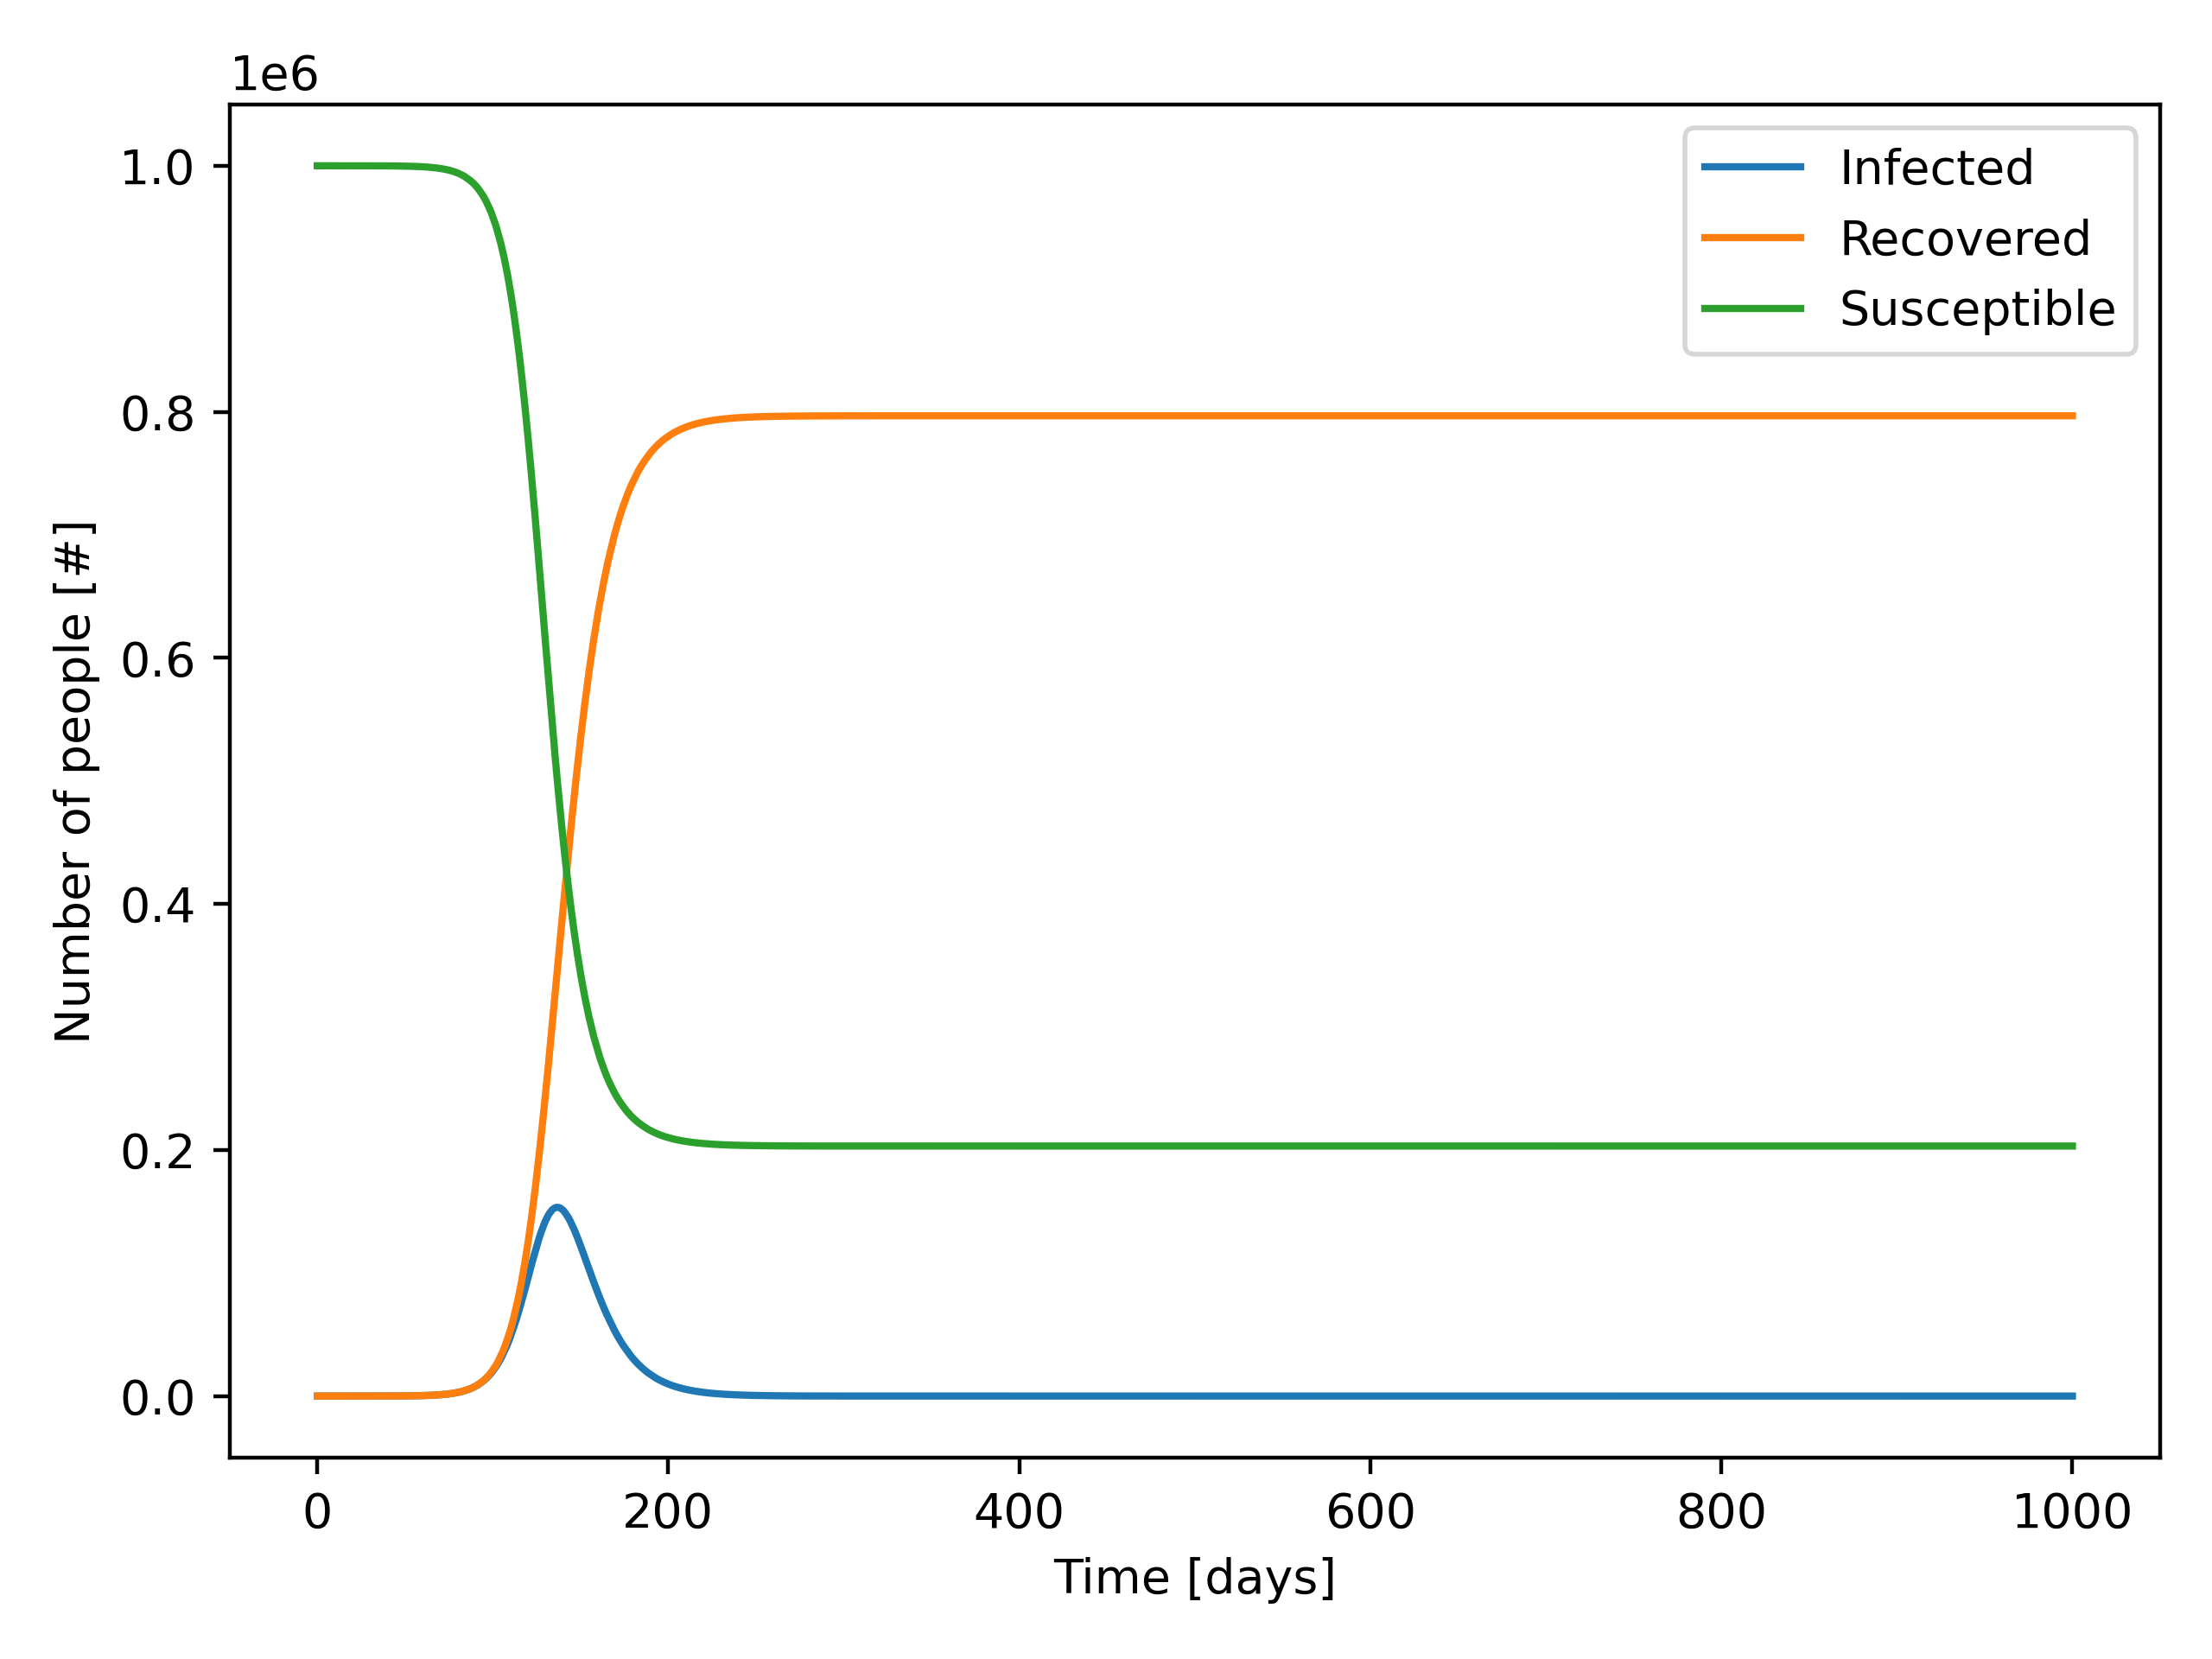
\includegraphics[width=0.5\textwidth]{Assignment_1_SIR/Report/Images/SIR_plot_dt0_001_pop1e6.png}
    \caption{Efficiency plot of the different model sizes.}
    \label{fig:Efficiency_plot}
\end{figure}
\FloatBarrier
\section{Source Code}
\label{sec:source}
\lstinputlisting[language=c++]{../fwc_parallel.cpp}

\end{document}